\section{Budget--Stability Sweep: Full Results}
\label{app:bsweep}

This appendix gives the full budget--stability sweep of
Section~\ref{sec:pilot-bsweep}, whose headline conclusions (agreement
rises with budget, $B = 20$ sits at the agreement floor, mean $L_1$ is a
confounded metric, and the budget should be set by the slowest-converging
family) are stated in the body. Here we report the per-call-seeding
negative result, the full table and curves, and the small-sample
artifact that a coarser probe produced.

\paragraph{Per-call seeding does not stabilize a collection.} The
stochastic transitions in the pilot were drawn at temperature $0.7$ with
no fixed sampling seed, so a natural first attempt is to forward a
per-call seed (derived from the planner's random state) to the LLM
server, which both Ollama and vLLM accept. We implemented this and
verified that an \emph{individual} call reproduces exactly at a matched
seed on our server. It does not, however, make a \emph{collection}
reproducible. The reason is structural: an MCTS search's sequence of LLM
calls is itself a function of the responses, because each response is the
next state and the next state determines the next prompt. A single
non-deterministic call early in the search (server-side batching and
floating-point reduction order make exact determinism fragile under load)
changes which node expands next, desynchronizes the seed-to-prompt
correspondence, and every downstream call then lands on a different
prompt. Measured on the same matched-seed setup, per-call seeding left
the cross-run $L_1$ statistically indistinguishable from the unseeded
baseline. One can seed the calls but not the tree they induce; the
seeding hook is retained because it makes single transitions reproducible
for debugging, not because it stabilizes collection.

\paragraph{Sweep design.} For a fixed initial state we ran $K = 20$
independent MCTS searches (different random seeds, hence independent
stochastic LLM transitions) at every budget
$B \in \{10, 20, 40, 80, 160\}$, on \texttt{multiply\_small} (a
low-ambiguity control) and \texttt{algebra\_toy\_1} (the high-ambiguity
family whose instability is the subject of
Section~\ref{sec:pilot-v3-v4}); the grid deliberately includes
$B = 20$, the pilot's own collection budget. Holding the start state
fixed across all runs isolates the visit-count estimator's own variance
from the trajectory cascade: any disagreement among the twenty
$\pimcts$ distributions is the estimator's sampling noise at that
budget, not a divergent trajectory. The stability statistic is
\emph{pairwise argmax agreement}: the probability that two independent
searches recommend the same verb, computed over all
$\binom{20}{2} = 190$ pairs, with bootstrap percentile confidence
intervals ($10{,}000$ resamples). Table~\ref{tab:pilot-bsweep} and
Figure~\ref{fig:pilot-bsweep} report the result.

\begin{table}[t]
\centering
\caption{Target stability versus search budget. For each problem and
budget $B$, twenty independent MCTS searches from the same fixed
initial state. ``mean max'' is the mean over runs of
$\max_a \pimcts(a\given s)$ (sharpness); ``$H$'' is mean entropy in
bits; ``pair.\ agree'' is the pairwise argmax agreement over all $190$
run pairs with a bootstrap $95\%$ CI; ``mean $L_1$'' is the mean
pairwise $L_1$ distance. $K=20$ per cell.}
\label{tab:pilot-bsweep}
\small
\begin{tabular}{@{}lrrrlr@{}}
\toprule
Problem & $B$ & mean max & $H$ (bits) & pair.\ agree [CI95] & mean $L_1$ \\
\midrule
\texttt{multiply\_small} &  10 & 0.35 & 1.92 & 0.41 [0.33, 0.61] & 0.259 \\
\texttt{multiply\_small} &  20 & 0.45 & 1.82 & 0.31 [0.30, 0.46] & 0.507 \\
\texttt{multiply\_small} &  40 & 0.65 & 1.42 & 0.52 [0.36, 0.81] & 0.643 \\
\texttt{multiply\_small} &  80 & 0.80 & 0.98 & 0.73 [0.56, 1.00] & 0.589 \\
\texttt{multiply\_small} & 160 & 0.88 & 0.68 & \textbf{0.81} [0.61, 1.00] & 0.456 \\
\texttt{algebra\_toy\_1} &  10 & 0.34 & 1.94 & 0.25 [0.22, 0.42] & 0.292 \\
\texttt{algebra\_toy\_1} &  20 & 0.38 & 1.90 & 0.32 [0.25, 0.49] & 0.376 \\
\texttt{algebra\_toy\_1} &  40 & 0.43 & 1.80 & 0.38 [0.29, 0.53] & 0.558 \\
\texttt{algebra\_toy\_1} &  80 & 0.49 & 1.73 & 0.46 [0.36, 0.66] & 0.580 \\
\texttt{algebra\_toy\_1} & 160 & 0.69 & 1.28 & \textbf{0.73} [0.56, 1.00] & 0.634 \\
\bottomrule
\end{tabular}
\end{table}

\begin{figure}[t]
\centering
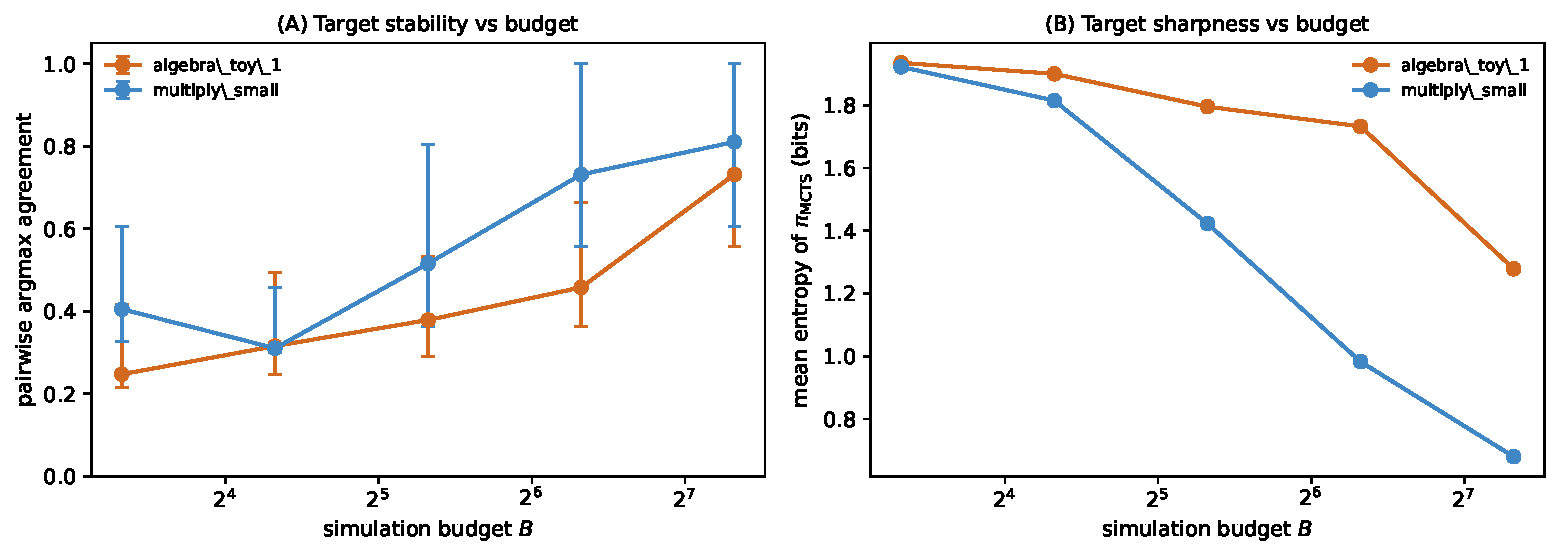
\includegraphics[width=\linewidth]{figures/b_sweep.pdf}
\caption{Budget--stability curves at $K = 20$ searches per cell.
\emph{Panel A:} pairwise argmax agreement versus simulation budget $B$
(log scale), with bootstrap $95\%$ CIs. Agreement rises with budget on
both problem families; the pilot's collection budget $B = 20$ sits at
the low-agreement floor of the grid. \emph{Panel B:} mean entropy of
$\pimcts$ versus $B$; sharpness improves monotonically. The two panels
together show why distributional distance is a misleading stability
metric: distributions sharpen steadily (B) while run-to-run agreement
is lowest precisely where distributions are flat-to-moderately-sharp
(A).}
\label{fig:pilot-bsweep}
\end{figure}

\paragraph{Detailed reading of the sweep.} Four things follow. First,
\emph{sharpness rises monotonically with the budget on both families}:
mean max-probability climbs from $0.34$--$0.35$ at $B = 10$ to $0.88$
(\texttt{multiply\_small}) and $0.69$ (\texttt{algebra\_toy\_1}) at
$B = 160$, and entropy falls in lockstep. The estimator concentrates
visits on the high-value verb as the budget grows, exactly as a
sampled-Bellman argument predicts.

Second, \emph{agreement rises with budget, and the pilot's $B = 20$
sits at the low-agreement floor}. Pairwise agreement reaches $0.81$
(\texttt{multiply\_small}) and $0.73$ (\texttt{algebra\_toy\_1}) at
$B = 160$, while the $B = 20$ cells ($0.31$ and $0.32$) are the two
lowest values in the grid outside algebra's $B = 10$. At the budget
the pilot actually collected with, two independent collections agree on
the training argmax less than a third of the time. The pilot's observed
target instability is therefore an expected property of its budget, not
an indictment of the framework. Convergence speed is family-dependent:
the easy family reaches $0.73$ by $B = 80$, the hard family needs
$B = 160$, so the budget that buys a stable target must be set by the
slowest-converging family.

Third, a methodological note we report because it would otherwise be
invisible: an earlier $K = 6$ pass over a coarser grid showed an
apparent agreement \emph{dip} at $B = 40$ on both families, suggesting a
``committed but disagreeing'' transition zone. At $K = 20$ that dip
dissolves on the hard family (the curve is strictly monotone) and
survives only weakly on the easy one (a $B = 20$ trough whose CI
overlaps its neighbors). Small-$K$ stability diagnostics can
manufacture qualitative structure; conclusions about the shape of the
budget--stability curve need $K$ well above what a quick probe
suggests.

Fourth, \emph{the mean-$L_1$ metric is confounded by sharpness and can
anti-correlate with true stability}. On \texttt{algebra\_toy\_1},
$L_1$ \emph{rises monotonically} ($0.29 \to 0.63$) while agreement also
rises: a single sharp minority run on a different verb costs roughly
$1.3$ in pairwise $L_1$, whereas two near-uniform distributions are
trivially close, so the metric punishes exactly the sharpening that
stability requires. The instability $L_1$ figures reported in the body
(the $0.553$ on matched-condition algebra at $B = 20$, for
example) are therefore a mixture of genuine disagreement and this
artifact, and recommended-verb agreement is the correct stability
signal. Relatedly, the \emph{target itself is budget-indexed} on the
hard family: algebra's modal verb flips from \textsc{ComputeSubexpr} at
$B = 80$ to \textsc{Backtrack} at $B = 160$ even as within-budget
agreement rises, because deeper trees back up different values.
``Stable target'' means stable \emph{at a fixed budget}; any
round-over-round comparison must hold $B$ constant.

The cost is real: each $B = 160$ search took roughly four minutes on our
hardware, so the pre-registered $B = 500$ implies a search on the order
of fifteen minutes. The convergence trend is the justification for
paying it. Two practical commitments follow for the larger study, beyond
those in Section~\ref{sec:pilot-lessons}: report the pairwise-agreement
diagnostic \emph{stratified by problem family} rather than pooled, and
set the heavy-search budget by the slowest-converging family rather than
the average.
